\begin{subfigure}{0.4\textwidth}
    \centering
    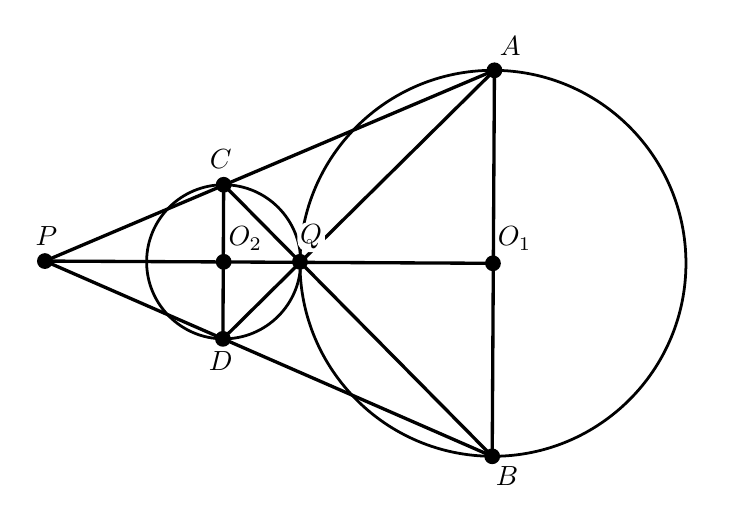
\begin{tikzpicture}[scale = 0.95]
        \clip(3.93,-4.43) rectangle (12.98,1.92);
        \draw [line width=1pt] (10.15,-1.23) circle (2.58cm);
        \draw [line width=1.2pt] (10.17,1.35)-- (10.14,-3.81);
        \draw [line width=1pt](6.55,-1.21) circle (1.03cm);
        \draw [line width=1.2pt] (10.17,1.35)-- (6.54,-2.24);
        \draw [line width=1.2pt] (10.14,-3.81)-- (6.55,-0.18);
        \draw [line width=1.2pt] (4.16,-1.2)-- (10.17,1.35);
        \draw [line width=1.2pt] (4.16,-1.2)-- (10.14,-3.81);
        \draw [line width=1.2pt] (6.55,-0.18)-- (6.54,-2.24);
        \draw [line width=1.2pt] (4.16,-1.2)-- (10.15,-1.23);
        \begin{scriptsize}
            \normalsize
            \fill [color=black] (10.15,-1.23) circle (3pt);
            \draw[color=black] (10.44,-0.9) node {$O_1$};
            \fill [color=black] (10.17,1.35) circle (3pt);
            \draw[color=black] (10.38,1.67) node {$A$};
            \fill [color=black] (10.14,-3.81) circle (3pt);
            \draw[color=black] (10.34,-4.07) node {$B$};
            \fill [color=black] (7.57,-1.21) circle (3pt);
            \draw[color=black] (7.72,-0.88) node[fill = white, rounded corners = 4pt, inner sep=1pt] {$Q$};
            \fill [color=black] (6.55,-1.21) circle (3pt);
            \draw[color=black] (6.84,-0.9) node {$O_2$};
            \fill [color=black] (6.55,-0.18) circle (3pt);
            \draw[color=black] (6.51,0.16) node {$C$};
            \fill [color=black] (6.54,-2.24) circle (3pt);
            \draw[color=black] (6.51,-2.54) node {$D$};
            \fill [color=black] (4.16,-1.2) circle (3pt);
            \draw[color=black] (4.18,-0.86) node {$P$};
        \end{scriptsize}
    \end{tikzpicture}
\end{subfigure}
\hspace{0.1\textwidth}
\begin{subfigure}{0.4\textwidth}
    \centering
    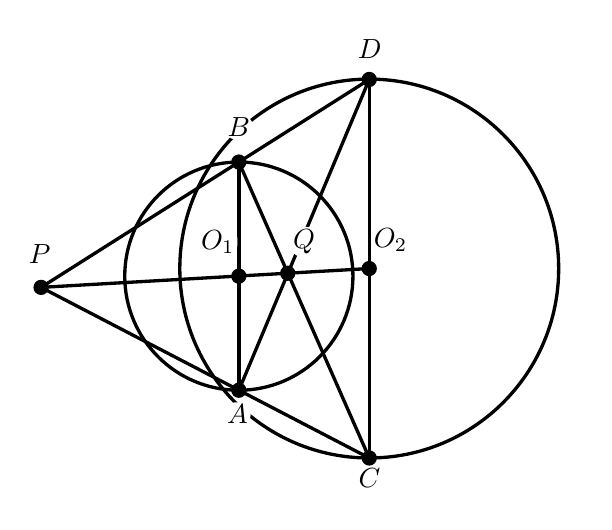
\begin{tikzpicture}[scale = 0.46]
        \clip(-0.43,-0.99) rectangle (14.92,12.11);
        \draw [line width=1.2pt] (5.4,5.25) circle (3.15cm);
        \draw [line width=1.2pt] (9,5.46) circle (5.23cm);
        \draw [line width=1.2pt] (-0.06,4.94)-- (9,0.23);
        \draw [line width=1.2pt] (-0.06,4.94)-- (9,10.68);
        \draw [line width=1.2pt] (-0.06,4.94)-- (9,5.46);
        \draw [line width=1.2pt] (5.4,2.1)-- (5.4,8.4);
        \draw [line width=1.2pt] (9,0.23)-- (9,10.68);
        \draw [line width=1.2pt] (5.4,2.1)-- (9,10.68);
        \draw [line width=1.2pt] (9,0.23)-- (5.4,8.4);
        \begin{scriptsize}
            \normalsize
            \fill [color=black] (5.4,5.25) circle (6pt);
            \draw[color=black] (4.82,6.2) node[fill = white, rounded corners = 4pt, inner sep=1pt] {$O_1$};
            \fill [color=black] (5.4,2.1) circle (6pt);
            \draw[color=black] (5.36,1.43) node[fill = white, rounded corners = 4pt, inner sep=1pt] {$A$};
            \fill [color=black] (5.4,8.4) circle (6pt);
            \draw[color=black] (5.4,9.36) node[fill = white, rounded corners = 4pt, inner sep=1pt] {$B$};
            \fill [color=black] (9,0.23) circle (6pt);
            \draw[color=black] (9.01,-0.33) node[fill = white, rounded corners = 4pt, inner sep=1pt] {$C$};
            \fill [color=black] (9,5.46) circle (6pt);
            \draw[color=black] (9.59,6.24) node[fill = white, rounded corners = 4pt, inner sep=1pt] {$O_2$};
            \fill [color=black] (9,10.68) circle (6pt);
            \draw[color=black] (9.01,11.53) node[fill = white, rounded corners = 4pt, inner sep=1pt] {$D$};
            \fill [color=black] (6.75,5.33) circle (6pt);
            \draw[color=black] (7.2,6.2) node[fill = white, rounded corners = 4pt, inner sep=1pt] {$Q$};
            \fill [color=black] (-0.06,4.94) circle (6pt);
            \draw[color=black] (-0.1,5.87) node[fill = white, rounded corners = 4pt, inner sep=1pt] {$P$};
        \end{scriptsize}
    \end{tikzpicture}
\end{subfigure}